\newcommand{\nonterminal}[1]{
    \langle \textbf{#1} \rangle
}

\newcommand{\m}[1]{
    {\color{OliveGreen}\bf#1}
}

\newcommand{\um}[1]{
    {\color{YellowOrange}\bf#1}
}

\newcommand{\nm}[1]{
    {\color{Maroon}\bf#1}
}
\chapter{Zoeken in strings}
\label{ch:zoeken_in_strings}
\begin{itemize}
    \item De gebruikte symbolen:

    \begin{table}[ht]
        \centering
        \begin{tabular}{c l}
            \hline
            Symbool & Betekenis \\
            \hline
            $\Sigma$ & Het gebruikte alfabet \\
            $\Sigma*$ & De verzameling strings van eindige lengte van letters uit $\Sigma$ \\
            d & Aantal karakters in $\Sigma$ \\
            P & Patroon (de tekst die gezocht wordt) \\
            p & Lengte van P \\
            T & De hele tekst waarin gezocht wordt\\
            t & lengte van T \\
            \hline
        \end{tabular}
    \end{table}

    \item We willen een bepaalde string (het patroon P) in een langere string (de tekst T) lokaliseren.
    \item We nemen aan dat we alle plaatsen zoeken waar dat patroon voorkoomt.
    \item We veronderstellen ook dat P en T in het inwendig geheugen opgeslaan zitten.

    \item In de voorbeelden worden volgende concrete informatie gebruikt:
    \begin{itemize}
        \item $\Sigma = \{A, C, G, T\}$
        \item $d = 4$
        \item $P = \texttt{GCAGAGCAG}$
        \item $p = 9$
        \item $T = \texttt{GCATCGCAGAGCAGAGTACAGCACG}$
        \item $t = 25$
    \end{itemize}

\end{itemize}


\section{Formele talen}
\begin{itemize}
    \item Een \textbf{formele taal} over een alfabet is een verzameling eindige strings over dat alfabet.
    \item Een formele taal wordt vrij vaag gedefinieerd (maar zien we niet in de cursus).
    \item Een formele taal kan op twee manieren gedefinieerd worden: via \textbf{generatieve grammatica's} of via \textbf{reguliere expressies}.
\end{itemize}

\subsection{Generatieve grammatica's}
\begin{itemize}
    \item Een \textbf{generatieve grammatica} is een methode om een taal te beschrijven.
    \item Er is een startsymbool dat getransformeerd kan worden tot een zin van de taal met behulp van substitutieregels.
    \item Buiten de karakters $\Sigma$ van het alfabet, is er ook nog een verzameling \textbf{niet-terminale symbolen}.
    \item Een niet-terminaal symbool wordt aangeduid als
        $$\nonterminal{\dots}$$
        waarin $\textbf{\dots}$ vervangen wordt door de naam van het niet-terminale symbool. 
    \item De verzameling alle strings uit $\Sigma$ vermengd met de niet-terminale symbolen is $\Xi$, en de daarbijhorende verzameling strings $\Xi*$.
    \item Een belangrijk geval zijn de \textbf{contextvrije grammatica's}.
    \begin{itemize}
        \item Er is op elk moment een string uit $\Xi*$.
        \item Als er geen niet-terminale symbolen meer zijn krijgt men een zin in de taal, anders kan men één niet-terminaal vervangen door een string uit $\Xi*$.
        \item De taal is contextvrij omdat de substitutie onafhankelijk is wat voor en achter de betreffende niet-terminaal staat.
        \item Een voorbeeld van een contextvrije grammatica:

        \begin{align*}
             \nonterminal{S} &::= \nonterminal{AB}\;|\;\nonterminal{CD} \\
             \nonterminal{AB} &::= a\nonterminal{AB}b\;|\;\epsilon \\
             \nonterminal{CD} &::= c\nonterminal{CD}c\;|\;\epsilon
        \end{align*}
        \begin{itemize}
            \item Hierbij is $\Sigma = \{ a, b, c, d \}$ en $\epsilon$ de lege string.
            \item Deze grammatica definieert als formele taal de verzameling van alle strings ofwel bestaande uit een rij 'a's gevolgd door een even lange rij 'b's ofwel bestaande uit een rij 'c's gevolgd door een even lange rij 'd's.    
            \item De afleiding van "cccddd":
            $$\nonterminal{S} \rightarrow \nonterminal{CD} \rightarrow c\nonterminal{CD}d \rightarrow cc\nonterminal{CD}dd \rightarrow ccc\nonterminal{CD}ddd \rightarrow cccddd$$
        \end{itemize}
    \end{itemize}
\end{itemize}

\subsection{Reguliere uitdrukkingen}
\begin{itemize}
    \item Een \textbf{reguliere uitdrukking} is ook een methode om een taal te beschrijven.
    \item Een reguliere uitdrukking, of \textit{regexp}, is een string over het alfabet $\Sigma = \{\sigma_0, \sigma_1, \cdots, \sigma_{d-1}\}$ aangevuld met de symbolen $\varnothing, \epsilon, *, (, )$ en $\bot$, gedefinieerd door
    \begin{align*}
        \nonterminal{Regexp} &::= \nonterminal{basis}\;|\;\nonterminal{samengesteld} \\
        \nonterminal{basis} &::= \sigma_0|\cdots|\sigma_{d-1}|\varnothing|\epsilon \\
        \nonterminal{samengesteld} &::= \nonterminal{plus}|\nonterminal{of}|\nonterminal{ster}\\
        \nonterminal{plus} &::= (\nonterminal{Regexp}\nonterminal{Regexp})\\
        \nonterminal{of} &::= (\nonterminal{Regexp}\bot\nonterminal{Regexp})\\
        \nonterminal{ster} &::= (\nonterminal{Regexp})*
    \end{align*}
    \item Elke regexp $R$ definieert een formele taal, Taal($R$).
    \item Een taal die door een regexp gedefinieerd kan worden heet een reguliere taal.
    \item De definitie van een regexp en reguliere taal is recursief:
    \begin{enumerate}
        \item $\varnothing$ is een regexp, met als taal de lege verzameling.
        \item De lege string $\epsilon$ is een regexp met als taal Taal($\epsilon$) = \{$\epsilon$\}.
        \item  Voor elke $a \in \Sigma$ is \quotes{a} een regexp, met als taal Taal(\quotes{a}) = \{\quotes{a}\}.
    \end{enumerate}
    \item Regexps kunnen gecombineerd worden via drie operaties:

    \begin{table}[ht]
        \centering
        \begin{tabular}{c c c}
            \hline
            Operatie & Regexp & Operatie op taal/talen \\
            \hline
            Concatenatie & (RS) & Taal($R$) $\cdot$ Taal($S$) \\
            Of & $(R|S)$ & Taal($R$) $\cup$ Taal($S$) \\
            Kleenesluiting & (R)* & Taal($R$)* \\
            \hline
        \end{tabular}

    \end{table}
    \item Vaak worden verkorte notaties gebruikt:
    \begin{itemize}
        \item \textbf{Minstens eenmaal herhalen}
        $$rr* \rightarrow r+$$
        \item \textbf{Optionele uitdrukking}
        $$r|\epsilon \rightarrow r?$$
        
        \item \textbf{Unies van symbolen}
        $$a|b|c \rightarrow [abc] $$
        $$a|b|\dots|z \rightarrow [a-z] $$

        
    \end{itemize}

    \item Regexps kunnen gelinkt worden met graafproblemen.
    \item \textbf{Stelling 1} Zij $G$ een gerichte multigraaf met verzameling takken $\Sigma$. Als $a$ en $b$ twee knopen van $G$ zijn dan is de verzameling $P_G(a, b)$ van paden beginnend in $a$ en eindigend in $b$ een reguliere taal over $\Sigma$.
    \item \textbf{Bewijs:}
    \begin{itemize}
        Via inductie op het aantal verbindingen $m$ van $G$.
        \item Als $m = 0$ dan
        $$P_G(a, b) = \begin{cases}
            \varnothing, \hbox{ als } a \neq b\\
            \{\epsilon\}, \hbox{ als } a = b 
        \end{cases}$$
        \item Breidt nu de graaf $G$ uit naar $G'$ door één verbinding toe te voegen.
        \begin{itemize}
            \item Een verbinding $v_{xy}$ van knoop $x$ naar knoop $y$, waarbij eventueel $x = y$.
            \item Alle paden van $a$ naar $b$ zijn één van de twee volgende vormen:
            \begin{enumerate}
                \item De paden die $v_{xy}$ niet bevatten. Deze vormen de reguliere taal $P_G(a, b)$.
                \item De paden die $v_{xy}$ wel bevatten. Deze verzameling wordt gegeven door
                $$P_G(a, x) \cdot \{v_{xy}\} \cdot (P_G(y, x) \cdot \{v_{xy}\})* \cdot P_G(y, b)$$

                Deze is bekomen uit reguliere talen en is dus regulier.
            \end{enumerate}
        \end{itemize}
    \end{itemize}
    \item 
\end{itemize}




\section{Variabele tekst}

\subsection{Een eenvoudige methode}
\begin{itemize}
    \item We zitten op een bepaalde positie $j$ in $T$.
    \item Vanaf $j$ wordt $T[j + i]$ met $P[i]$ vergeleken voor $0 < i \leq p$.
    \begin{enumerate}
        \item Het eerste geval komt voor wanneer $T[j + i] \neq P[i]$, voor $i \leq p$, en het patroon dus niet gevonden is op positie $j$ in $T$.
        \item Het tweede geval komt dan voor wanneer het patroon wel gevonden is op positie $j$ in $T$.
    \end{enumerate}
    \item Voor willekeurige strings zal $T[j]$ vaak verschillen van $P[0]$.
    \begin{itemize}
        \item Op veel posities $j$ zal de karaktervergelijking na één positie dan stoppen.
    \end{itemize}
    \item De \textbf{gemiddelde uitvoeringstijd} is $O(t)$.
    \item Het \textbf{slechtste geval} is $O(tp)$.
\end{itemize}

\begin{table}[ht]
    \centering
    \scalebox{0.7}{
        %GCATCGCAGAGCAGAGTACAGCACG
    \begin{tabular}{|c |c c c c c c c c c c c c c c c c c c c c c c c c c|}
        \hline
        j & 0 & 1 & 2 & 3 & 4 & 5 & 6 & 7 & 8 & 9 & 10 &11&12 &13 &14 &15 &16 &17 &18 &19 &20 &21 &22 &23&24\\
       
        T & G & C & A & T & C & G & C & A & G & A & G & C & A & G & A & G & T & A & C & A & G & C & A & C & G\\
          \hline
          &\m{G}&\m{C}&\m{A}&\nm{G}& A & G & C & A & G &   &   &   &   &   &   &   &   &   &   &   &   &   &   &   &  \\
          &   &\nm{G}& C & A & G & A & G & C & A & G &   &   &   &   &   &   &   &   &   &   &   &   &   &   &  \\
          &   &   &\nm{G}& C & A & G & A & G & C& A & G &   &   &   &   &   &   &   &   &   &   &   &   &   &  \\
          &   &   &   &\nm{G}& C & A & G & A & G & C& A & G &   &   &   &   &   &   &   &   &   &   &   &   &  \\
          &   &   &   &   &\nm{G}& C & A & G & A & G & C& A & G &   &   &   &   &   &   &   &   &   &   &   &  \\
          &   &   &   &   &   &\m{G}&\m{C}&\m{A}&\m{G}&\m{A}&\m{G}&\m{C}&\m{A}&\m{G}&   &   &   &   &   &   &   &   &   &   &  \\
          &   &   &   &   &   &   &\nm{G}& C & A & G & A & G & C& A & G &   &   &   &   &   &   &   &   &  &    \\
          &   &   &   &   &   &   &   &\nm{G}& C & A & G & A & G& C & A & G &   &   &   &   &   &   &   &   &    \\
          &   &   &   &   &   &   &   &   &\m{G}&\nm{C}& A & G & A & G& C & A & G &   &   &   &   & &   &   &     \\
          &   &   &   &   &   &   &   &   &   &\nm{G}& C & A & G & A & G& C & A & G &   &   &   &   &   &  &    \\
          &   &   &   &   &   &   &   &   &   &   &\m{G}&\m{C}&\m{A}&\m{G}&\m{A}&\m{G}&\nm{C}& A & G &   &   &  &  &   &    \\
          &   &   &   &   &   &   &   &   &   &   &   &\nm{G}& C & A & G & A & G & C& A & G &   &   &   &  &   \\
          &   &   &   &   &   &   &   &   &   &   &   &    &\nm{G}&C & A & G & A & G& C & A & G &   &   &  &   \\
          &   &   &   &   &   &   &   &   &   &   &   &   &  &\m{G}&\nm{C}& A & G & A & G& C & A & G &   &   &    \\
          &   &   &   &   &   &   &   &   &   &   &   &   &  &   &\nm{G}& C & A & G & A & G & C& A & G &   &  \\
          &   &   &   &   &   &   &   &   &   &   &   &   &  &  &    &\m{G}&\nm{C}& A & G & A & G & C& A & G &  \\
          &   &   &   &   &   &   &   &   &   &   &   &   &  &  &  &  &\nm{G}& C & A & G & A & G & C& A & G  \\
          \hline   
    \end{tabular}
    }
\end{table}



\subsection{Knuth-Morris-Pratt}
\subsubsection{De prefixfunctie}
\begin{itemize}
    \item Gegeven een string $P$ en index $i$ met $i \leq p$.
    \item Een string $Q$ kan voor $i$ op $P$ gelegd woorden als $i \geq q$ en als $Q$ overeenkomt met de even lange deelstring van $P$ endigend voor $i$.
    \begin{itemize}
        \item De index $i$ wijst naar de plaats \textit{voorbij} de deelstring, niet naar de laatste letter van de deelstring.
    \end{itemize}
    \item De prefixfunctie $q(i)$ van een string $P$ bepaalt voor elke stringpositie $i$, $1 \leq i \leq p$, de lengte van de langste prefix van $P$ met lengte kleiner dan $i$ dat we voor $i$ kunnen leggen.

    \item Volgende eigenschappen gelden:
    \begin{itemize}
        \item $q(0) = -$ (niet gedefinieerd)
        \item $q(1) = 0$
        \item $q(i) < i$
        \item $q(i + 1) \leq q(i) + 1$
    \end{itemize}
    \item De waarde van $q(i + 1)$ kan bepaald worden als de waarden van de vorige posities gekend zijn.
    $$q(i + 1) = \begin{cases}
        q(i) + 1 & \hbox{ als } P[q(i)] = P[i]  \\
        q(q(i)) + 1 & \hbox{ als } P[q(q(i))] = P[i] \\
        q(q(q(i))) + 1 & \hbox{ als } P[q(q(q(i)))] = P[i] \\
        \cdots \\
        0 & \hbox { als } q(q(q(....))) = 0
    \end{cases}$$

    \begin{itemize}
        \item De waarden van de prefixfunctie voor $P = $ \texttt{ANOANAANOANO} zijn als volgt:
        \begin{itemize}
            \item Voor $i = 2$ geldt $q(i) = 0$:
            \begin{itemize}
                \item $P[q(1)] = P[1]\;?\;\rightarrow P[0] = P[1]\;?\;\rightarrow A \neq N$
                \item $q(2) = 0$
            \end{itemize} 
            \item Voor $i = 4$ geldt $q(i) = 1$:
            \begin{itemize}
                \item $P[q(3)] = P[3]\;?\;\rightarrow P[0] = P[3]\;?\;\rightarrow A = A$
                \item $q(4) = q(3) + 1 = 0 + 1 = 1$
            \end{itemize}
            \item Voor $i = 12$ geldt $q(i) = 3$:
            \begin{itemize}
                \item $P[q(11)] = P[11]\;?\;\rightarrow P[5] = P[11]\;?\;\rightarrow A \neq O$
                \item $P(q(5)) = P[11]\;?\;\rightarrow P[2] = P[11]\;?\;\rightarrow O = O$
                \item $q(12) = q(5) + 1 = 2 + 1 = 3$
            \end{itemize}
        \end{itemize}

        \begin{table}[ht]
            \centering
            \begin{tabular}{l | c c c c c c c c c c c c c}
                     & A & N & O & A & N & A & A & N & O & A  & N  & O  & - \\
                     \hline
                i    & 0 & 1 & 2 & 3 & 4 & 5 & 6 & 7 & 8 & 9 & 10 & 11 & 12  \\
                q(i) & - & 0 & 0 & 0 & 1 & 2 & 1 & 1 & 2 & 3  & 4  & 5 & 3 
            \end{tabular}
        \end{table}
    \end{itemize}
    \item De prefixwaarden worden dus voor stijgende $i$ berekend.
    \item Wat is de \textbf{efficiëntie}?
    \begin{itemize}
        \item Er moeten $p$ prefixwaarden berekend worden.
        \item De recursierelatie wordt ook maar $p-1$ herhaald voor de voltallige bepaling van de prefixfunctie.
        \item De methode is $\Theta(p)$.
    \end{itemize}
\end{itemize}

\subsubsection{Een eenvoudige lineaire methode}
\begin{itemize}
    \item Stel een string samen bestaande uit $P$ gevolgd door $T$, gescheiden door een speciaal karakter dat in niet in beide strings voorkomt.
    \item Bepaal de prefixfunctie van deze nieuwe string, in $\Theta(n + p)$.
    \item Als de prefixwaarde van een positie $i$ gelijk is aan $p$, werd $P$ gevonden, beginnend bij index $i - p$ in $T$.
\end{itemize}


\subsubsection{Het Knuth-Morris-Prattalgoritme}
\begin{itemize}
    \item Ook een lineaire methode, maar is efficiënter.
    \item Stel dat $P$ op een bepaalde beginpositie vergeleken wordt met $T$, en dat er geen overeenkomst meer is tussen $P[i]$ en $T[j]$.
    \begin{itemize}
        \item Als $i = 0$, dan wordt $P$ één positie naar rechts geschoven en begint het vergelijken met $T$ weer bij $P[0]$.
        \item Als $i > 0$, dan is er een prefix van $P$ met lengte $i$ gevonden, dat we voor $j$ op $T$ kunnen leggen.
        \begin{itemize}
            \item Verschuif $P$ met een stap $s$ kleiner dan $i$.
            \item Er is nu een overlapping tussen het begin van $P$ en het prefix van $P$ dat we in $T$ gevonden hebben.
            \item De overlapping heeft lengte $i - s$.
            \item De overlappende delen moeten wel overeenkomen.
            \item De kleinste waarde van $s$ waarbij dit mogelijk is, is $s = i - q(i)$.
            \item Verschuif $P$ met $s$ en vergelijk verder vanaf $T[j]$ en $P[q(i)]$.
        \end{itemize}
        \begin{table}[ht]
            \centering
            \begin{tabular}{l | c c c c c c c c c c}
                i   & 0 & 1 & 2 & 3 & 4 & 5 & 6 & 7 & 8 & 9\\
                P   & G & C & A & G & A & G & C & A & G & - \\
                    \hline
                q(i) & -1 & 0 & 0 & 0 & 1 & 0 & 1 & 2 & 3 & 4 \\
                s   & 1 & 1 & 2 & 3 & 3 & 5 & 5 & 5 & 5 & 5
            \end{tabular}
            \caption{Het patroon $P = \texttt{GCAGAGCAG}$, de bijhorende prefixfunctie $q(i)$ en de $s$-waarden.}
            \label{table:kmp1}
        \end{table}

        \begin{table}[ht]
            \centering   
            \scalebox{0.6}{
            \begin{tabular}{|c c |c c c c c c c c c c c c c c c c c c c c c c c cc |}
                \hline
                \multicolumn{2}{|r|}{j} & 0 & 1 & 2 & 3 & 4 & 5 & 6 & 7 & 8 & 9 & 10 &11&12 &13 &14 &15 &16 &17 &18 &19 &20 &21 &22 &23&24\\    
                \multicolumn{2}{|r|}{T}  & G & C & A & T & C & G & C & A & G & A & G&C & A & G & A & G & T & A & C & A & G & C & A & C & G\\
                  \hline
                  $i - q(i)$ & sprong   &  &   &  &  &  &  &  &   &   &   &   &   &   &   &   &   &   &   &   &   &   &   &&&  \\
                   3 - 0     &   3      &\m{G}&\m{C}&\m{A}&\nm{G}&A&G&C&A&G&&&&&&&&&&&&&&&& \\
                   0 - (-1)  &   1      &&&&\nm{G}&C&A&G&A&G&C&A&G&&&&&&&&&&&&& \\
                   0 - (-1)  &   1      &&&&&\nm{G}&C&A&G&A&G&C&A&G&&&&&&&&&&&& \\
                   9 - 4  &   5         &&&&&&\m{G}&\m{C}&\m{A}&\m{G}&\m{A}&\m{G}&\m{C}&\m{A}&\m{G}&&&&&&&&&&& \\
                   6 - 1  &   5         &&&&&&&&&&&\m{G}&\m{C}&\m{A}&\m{G}&\m{A}&\m{G}&\nm{C}&A&G&&&&&& \\
                   1 - 0  &   1         &&&&&&&&&&&&&&&&\m{G}&\nm{C}&A&G&A&G&C&A&G& \\
                   1 - 0  &   1         &&&&&&&&&&&&&&&&&\nm{G}&C&A&G&A&G&C&A&G \\
                  \hline   
            \end{tabular}
            }
            \caption{Een eerste versie van het Knuth-Morris-Prattalgoritme, , waarbij $s = i - q(i)$.}
            \label{table:kmpex1}
        \end{table}

    \end{itemize}
    \item In tabel \ref{table:kmpex1} kan opgemerkt worden dat bij de verschuiving, waarbij de fout op $T[16] = T$ veroorzaakt door het verkeerde karakter $C$, er opnieuw een $C$ vergeleken wordt (Dit geldt niet voor $T[3]$ en het verkeerde karakter $G$ omdat de verschuiving naar de eerste letter van het patroon is). 
    \item Er is een \textbf{bijkomende voorwaarde}: de verschuiving $s$ is enkel zinvol als $P[i - s] \neq P[i]$.
    \item Op basis van $q(i)$ wordt een nieuwe functie $q'(i)$ gedefinieerd, die een zinvolle verschuiving $s = i - q'(i)$ geeft, zodanig dat $P[i - s] \neq P[i]$.

    $$q'(i) = \begin{cases}
        0 & \hbox{ als } q(i) = 0  \\
        q(i) & \hbox{ als } q[i] \neq 0 \hbox{ en } P[q(i) + 1] \neq P[i + 1] \\
        q'(q(i)) & \hbox{ als } q[i] \neq 0 \hbox{ en } P[q(i) + 1] = P[i + 1] \\
    \end{cases}$$
    %
    \begin{table}[ht]
        \centering
        \begin{tabular}{l | c c c c c c c c c c}
            i   & 0 & 1 & 2 & 3 & 4 & 5 & 6 & 7 & 8 & 9\\
            P   & G & C & A & G & A & G & C & A & G & - \\
                \hline
            q(i) & -1 & 0 & 0 & 0 & 1 & 0 & 1 & 2 & 3 & 4 \\
            q'(i) & -1 & 0 & 0 & 0 & 1 & 0 & 0 & 0 & 0 & 4 \\
            s   & 1 & 1 & 2 & 3 & 3 & 5 & 6 & 7 & 8 & 5
        \end{tabular}
        \caption{Het patroon $P = \texttt{GCAGAGCAG}$, de nieuwe prefixfunctie $q'(i)$ en de nieuwe $s$-waarden.}
        \label{table:kmp2}
    \end{table}

    \begin{table}[ht]
        \centering   
        \scalebox{0.6}{
        \begin{tabular}{|c c |c c c c c c c c c c c c c c c c c c c c c c c cc |}
            \hline
            \multicolumn{2}{|r|}{j} & 0 & 1 & 2 & 3 & 4 & 5 & 6 & 7 & 8 & 9 & 10 &11&12 &13 &14 &15 &16 &17 &18 &19 &20 &21 &22 &23&24\\    
            \multicolumn{2}{|r|}{T}  & G & C & A & T & C & G & C & A & G & A & G&C & A & G & A & G & T & A & C & A & G & C & A & C & G\\
              \hline
              $i - q'(i)$ & sprong   &  &   &  &  &  &  &  &   &   &   &   &   &   &   &   &   &   &   &   &   &   &   &&&  \\
               3 - 0     &   3      &\m{G}&\m{C}&\m{A}&\nm{G}&A&G&C&A&G&&&&&&&&&&&&&&&& \\
               0 - (-1)  &   1      &&&&\nm{G}&C&A&G&A&G&C&A&G&&&&&&&&&&&&& \\
               0 - (-1)  &   1      &&&&&\nm{G}&C&A&G&A&G&C&A&G&&&&&&&&&&&& \\
               9 - 4  &   5         &&&&&&\m{G}&\m{C}&\m{A}&\m{G}&\m{A}&\m{G}&\m{C}&\m{A}&\m{G}&&&&&&&&&&& \\
               6 - 0  &   6         &&&&&&&&&&&\m{G}&\m{C}&\m{A}&\m{G}&\m{A}&\m{G}&\nm{C}&A&G&&&&&& \\
               1 - 0  &   1         &&&&&&&&&&&&&&&&&\nm{G}&C&A&G&A&G&C&A&G \\
              \hline   
        \end{tabular}
        }
        \caption{De tweede versie van het Knuth-Morris-Prattalgoritme, waarbij $s = i - q'(i)$.}
        \label{table:kmpex1}
    \end{table}

\end{itemize}


\subsection{Boyer-Moore}
\begin{itemize}
    \item Dit algoritme is een \textbf{variant} van het Knuth-Morris-Prattalgoritme.
    \alert Het patroon wordt van achter naar voor overlopen bij het vergelijken met de tekst.
    \item Er worden \textbf{twee heuristieken} gebruikt die grotere verschuivingen mogelijk maakt. Het maximum van de twee heuristieken wordt dan gebruikt als verschuiving:
    \begin{enumerate}
        \item \textbf{De heuristiek van het verkeerde karakter}.
        \item \textbf{De heuristiek van het juiste suffix}.
    \end{enumerate}
\end{itemize}

\subsubsection{De heuristiek van het verkeerde karakter}
\begin{itemize}
    \item Het tekstkarakter waar een fout voorkomt wordt $f$ genoemd (het verkeerde karakter in de tekst $T$).
    \item Als $T$ ook dit karakter bevat, op een andere positie, kan $P$ naar rechts verschoven worden.
    \item Om de verschuiving te bepalen wordt \textbf{de meest rechtse positie} $i$, links van $p - 1$ in $P$ van elk karakter in het alfabet bijgehouden.
    \begin{itemize}
        \item Dit wordt geïmplementeerd als een tabel, MRP genaamd, geïndexeerd op de karakters van het alfabet (tabel \ref{table:bm2}).
        \begin{table}[ht]
            \centering
            \begin{tabular}{l | cccc}
                $f$ & A & C & G & T \\
                \hline
                $MRP[f]$    & 7 & 6 & 5 & -1
            \end{tabular}
            \caption{De MRP-tabel voor $P = \texttt{GCAGAGCAG}$. De waarden voor $A$ en $C$ zijn vanzelfsprekend. De waarde van $G$ is niet 8, omdat dat sowieso het eerste karakter is dat vergeleken wordt, en telt niet mee. Een karakter dat niet in het patroon voorkomt krijgt de waarde -1.}
            \label{table:bm2}
        \end{table}

        \item Het volstaat nu om de waarde $k = MRP[f]$ op te zoeken, waarbij $f$ het foute karakter in $T$ is, op positie $i$ in $P$, en $P$ te verschuiven over $i - k$ posities. 
        \begin{itemize}
            \alert In het geval dat $i - k < 0$, dan bedraagt de verschuiving $1$ positie.
        \end{itemize}
    \end{itemize}

    \begin{table}[ht]
        \centering   
        \scalebox{0.6}{
        \begin{tabular}{|c c c |c c c c c c c c c c c c c c c c c c c c c c c c c|}
            \hline
            \multicolumn{3}{|r|}{j} & 0 & 1 & 2 & 3 & 4 & 5 & 6 & 7 & 8 & 9 & 10 &11&12 &13 &14 &15 &16 &17 &18 &19 &20 &21 &22 &23&24\\    
            \multicolumn{3}{|r|}{T}  & G & C & A & T & C & G & C & A & G & A & G&C & A & G & A & G & T & A & C & A & G & C & A & C & G\\
              \hline
             f& $i - k$ & sprong   &  &   &  &  &  &  &  &   &   &   &   &   &   &   &   &   &   &   &   &   &   &   &&&  \\
             C & $4 - 6$&   1      &G&C&A&G&\nm{A}&\m{G}&\m{C}&\m{A}&\m{G}&&&&&&&&&&&&&&&&  \\
             A & $8 - 7$&   1      &&G&C&A&G&A&G&C&A&\nm{G}&&&&&&&&&&&&&&&  \\
             G & $6 - 5$&   1      &&&G&C&A&G&A&G&\nm{C}&\m{A}&\m{G}&&&&&&&&&&&&&&  \\
             C & $8 - 6$&   2      &&&&G&C&A&G&A&G&C&A&\nm{G}&&&&&&&&&&&&&  \\
             / &    /   &   1      &&&&&&\m{G}&\m{C}&\m{A}&\m{G}&\m{A}&\m{G}&\m{C}&\m{A}&\m{G}&&&&&&&&&&&  \\
             A & $8 - 7$&  1       &&&&&&&G&C&A&G&A&G&C&A&\nm{G}&&&&&&&&&&  \\
             G & $6 - 5$&  2       &&&&&&&&G&C&A&G&A&G&\nm{C}&\m{A}&\m{G}&&&&&&&&&  \\
             A & $8 - 7$&  1       &&&&&&&&&&G&C&A&G&A&G&C&A&\nm{G}&&&&&&&  \\
             C & $8 - 6$&  2       &&&&&&&&&&&G&C&A&G&A&G&C&A&\nm{G}&&&&&&  \\
             A & $5 - 6$&  1       &&&&&&&&&&&&&G&C&A&G&A&\nm{G}&\m{C}&\m{A}&\m{G}&&&&  \\
             C & $8 - 6$&  2       &&&&&&&&&&&&&&G&C&A&G&A&G&C&A&\nm{G}&&&  \\
             C & $8 - 6$&  2       &&&&&&&&&&&&&&&&G&C&A&G&A&G&C&A&\nm{G}&  \\
            \hline   
        \end{tabular}
        }
        \caption{Het Boyer-Moore algoritme, enkel gebruik makend van de oorspronkelijke heuristiek van het verkeerde karakter.}
    \end{table}
    \item Er zijn \textbf{drie varianten} van deze heuristiek:
    \begin{enumerate}
        \item \textbf{Uitgebreide heuristiek van het verkeerde karakter}.
        \begin{itemize}
            \item De MRP-tabel wordt uitgebreidt, zodat $MRP[f]$ de positie $j$ teruggeeft, \textbf{links} van foutpositie $i$ in het patroon.
            \item Hiervoor is een tweedimensionale tabel nodig en is in het algemeen een vrij slechte uitbreiding.

        \end{itemize}
        \item \textbf{Variant van Horspool}.
        \begin{itemize}
            \item Dezelfde MRP-tabel als in de oorspronkelijke versie wordt gebruikt.
            \item Bij en fout op tekstpositie $m$ (positie waarbij $P[0]$ overeenkomt met $T$) en patroonpositie $i$, wordt $P$ zodanig opgeschoven zodanig dat $T[m + p - 1] = P[p - 1]$.
            \item Zoek de positie van de meest rechtste positie van het karakter van $T[m + p - 1]$: $k = MRP[T[m + p - 1]]$.
            \item De verschuiving van $P$ bedraagt bij een fout dan altijd $p - 1 - k$.
            \begin{itemize}
                \good Verschuiving is onafhankelijk van patroonpositie $i$.
            \end{itemize}
            \item Als deze variant gebruikt wordt, wordt de tweede heuristiek niet gebruikt, wat in het slechtste geval dus $O(pt)$ oplevert.
            \begin{table}[ht]
                \centering   
                \scalebox{0.5}{
                    
                \begin{tabular}{|c c c c |c c c c c c c c c c c c c c c c c c c c c c c cc |}
                    \hline
                    \multicolumn{4}{|r|}{j} & 0 & 1 & 2 & 3 & 4 & 5 & 6 & 7 & 8 & 9 & 10 &11&12 &13 &14 &15 &16 &17 &18 &19 &20 &21 &22 &23&24\\    
                    \multicolumn{4}{|r|}{T}  & G & C & A & T & C & G & C & A & G & A & G&C & A & G & A & G & T & A & C & A & G & C & A & C & G\\
                      \hline
                     $m$ & $T[m + p - 1]$& $p - 1 - k$ & sprong   &  &   &  &  &  &  &  &   &   &   &   &   &   &   &   &   &   &   &   &   &   &   && & \\
                     0& G&  $9 - 1 - 5$  & $3$  &G&C&A&G&\nm{A}&\m{G}&\m{C}&\m{A}&\m{G}&&&&&&&&&&&&&&&&  \\
                     3& C&  $9 - 1 - 6$  & $2$  &&&&G&C&A&G&A&G&C&A&\nm{G}&&&&&&&&&&&&& \\
                     5& /&  /  & $1$            &&&&&&\m{G}&\m{C}&\m{A}&\m{G}&\m{A}&\m{G}&\m{C}&\m{A}&\m{G}&&&&&&&&&&&  \\
                     6& A&  $9 - 1 - 7$  & $1$  &&&&&&&G&C&A&G&A&G&C&A&\nm{G}&&&&&&&&&& \\
                     7& G&  $9 - 1 - 5$  & $3$  &&&&&&&&G&C&A&G&A&G&\nm{C}&\m{A}&\m{G}&&&&&&&&& \\
                     10& C&  $9 - 1 - 6$  & $2$ &&&&&&&&&&&G&C&A&G&A&G&C&A&\nm{G}&&&&&& \\
                     12& G&  $9 - 1 - 5$  & $3$ &&&&&&&&&&&&&G&C&A&G&A&\nm{G}&\m{C}&\m{A}&\m{G}&&&&\\
                     15& C&  $9 - 1 - 6$  & $2$  &&&&&&&&&&&&&&&&G&C&A&G&A&G&C&A&\nm{G}&\\
                      \hline   
                \end{tabular}
                }
                \caption{Het Boyer-Moore algoritme: Horspool variant.}
            \end{table}
        \end{itemize}
        \item \textbf{Variant van Sunday}.
        \begin{itemize}
            \item ???
        \end{itemize}
    \end{enumerate}
    
\end{itemize}

\subsubsection{De heuristiek van het juiste suffix}
\begin{itemize}
    \item Hier wordt enkel de versie van de \textbf{originele Boyer-Moore} methode besproken, dus niet de varianten van Horspool of Sunday.
    \item In vele gevallen kan $f$ aan de rechterkant van foutpositie $i$ voorkomen, zodat $i - j < 0$, en er dus maar een verschuiving van 1 positie mogelijk is.
    \item Op positie $i$ in $P$ vinden we een verkeerd karakter $f$ in $T$.
    \item Er is dus een \textbf{suffix} van $P$ in $T$, met lengte $p - i - 1$.
    \item We willen weten of dit suffix $s$ nog ergens in $P$ voorkomt.
    \begin{itemize}
        \item Als er meerdere plaatsen zijn waar $s$ in $P$ voorkomt, wordt de meeste rechtse genomen.
        \item Suffixen kunnen overlappen.
    \end{itemize}
    \item We willen dus de meeste rechtste positie $j$ in $P$, waarbij $j \leq i$ waar een deelstring $s' = s$ begint.
    \item Analoog aan de prefixfunctie, is er nu een suffixfunctie $s(j)$:
    \begin{itemize}
        \item Voor elke index $j$ in $P$ wordt de lengte van het grootste suffix van $P$ bijgehouden, dat op index $j$ begint.
        \item De suffixwaarden is het omgekeerde van de prefixtabel voor het omgekeerde patroon $P$.
        \item De grootste waarde voor $j$ waarvoor $s(j) = p - i - 1$ is de waarde voor $k$.
        \item Een verschuiving $v[i]$ voor foutpositie $i$ in $P$ is dan $i + 1 - k$. Als $k$ niet gedefinieerd is dan is $v[i] = p - s[0]$.
    \end{itemize}

    \begin{table}[ht]
        \centering
        \begin{tabular}{l | c c c c c c c c c}
            $i$   & 0 & \um{1} & 2 & 3 & \nm{4} & \m{5} & 6 & 7 & \textbf{8} \\
            $P$   & G & C & A & G & A & G & C & A & G \\
                \hline
            $s(i)$ & 4 & \um{3} & 2 & 1 & \nm{2} & \m{1} & 0 & 0 & \textbf{0} \\
            $p - i - 1$ & 8 & 7 & 6 & 5 & 4 & \um{3} & \nm{2} & \m{1} & \textbf{0} \\
            $k$    & -  & -  & -  & -  &  - &  \um{1}  & \nm{4}   &  \m{5} & \textbf{8} \\
            $i + 1 - k$ & - & - & - & - & - & 5 & 3 & 3 & 1 \\
            $v[i]$ & 5 & 5 & 5 & 5 & 5 & 5 & 3  & 3 & 1
        \end{tabular}
        \caption{De waarden voor $k$ worden als volgt berekent: zoek de grootste $i$ zodanig dat $s(i) = p - i - 1$. De gekleurde cijfers in de tabel toont voor elke $k$ de relatie met index $i$ en $s(i) = p - i - 1$.}
        \label{table:bm3}
    \end{table}
    \item Er zijn \textbf{drie speciale gevallen} die zich kunnen voordoen:
    \begin{enumerate}
        \item \textbf{Het patroon $P$ werd gevonden}.
        \begin{itemize}
            \item Er is geen foutief patroonpositie ($i = -1$) en het juiste suffix is nu $P$ zelf.
            \item Toch mogen er geen  $p$ posities opgeschoven worden, want een nieuwe $P$ in $T$ kan de vorige gedeeltelijk overlappen.
            \item De overlapping is het langst mogelijke suffix van $P$, korter dan $p$.
            \item De verschuiving is dus $v[-1] = p - s[0]$ (virtueel tabelelement, kan geïmplementeerd worden als constante).
        \end{itemize}
        \item \textbf{Er is geen juist suffix}.
        \begin{itemize}
            \item Als $i = p - 1$, dan is er geen juist suffix.
            \item Er is geen waarde voor de verschuiving, dus de waarde van de eerste heuristiek moet gebruikt worden.
        \end{itemize}
        \item \textbf{Het juiste suffix komt niet meer in $P$ voor}.
        \begin{itemize}
            \item Er is geen index $j$ gevonden waarvoor $s(j) = p - i - 1$.
            \item De verschuiving is opnieuw $v[i] = p - s[0]$ voor $0 < i < p$.
        \end{itemize}
    \end{enumerate}
\end{itemize}

\subsection{Onzekere algoritmen}
\begin{itemize}
    \item Algoritmen die een zekere waarschijnlijkheid hebben om een geheel foutief resultaat te geven.
    \item Zulke algoritmen worden ook \textbf{Monte Carloalgoritmen} genoemd.
    \item Er zijn redenen waarom zulke algoritmen toch nuttig kunnen zijn;
    \begin{enumerate}
        \item Zulke algoritmen zijn vaak sneller.
        \begin{itemize}
            \item Een voorbeeld is een \textbf{Bloomfilter} (figuur \ref{fig:bloomfilter}).
            \begin{figure}[ht]
                \centering
                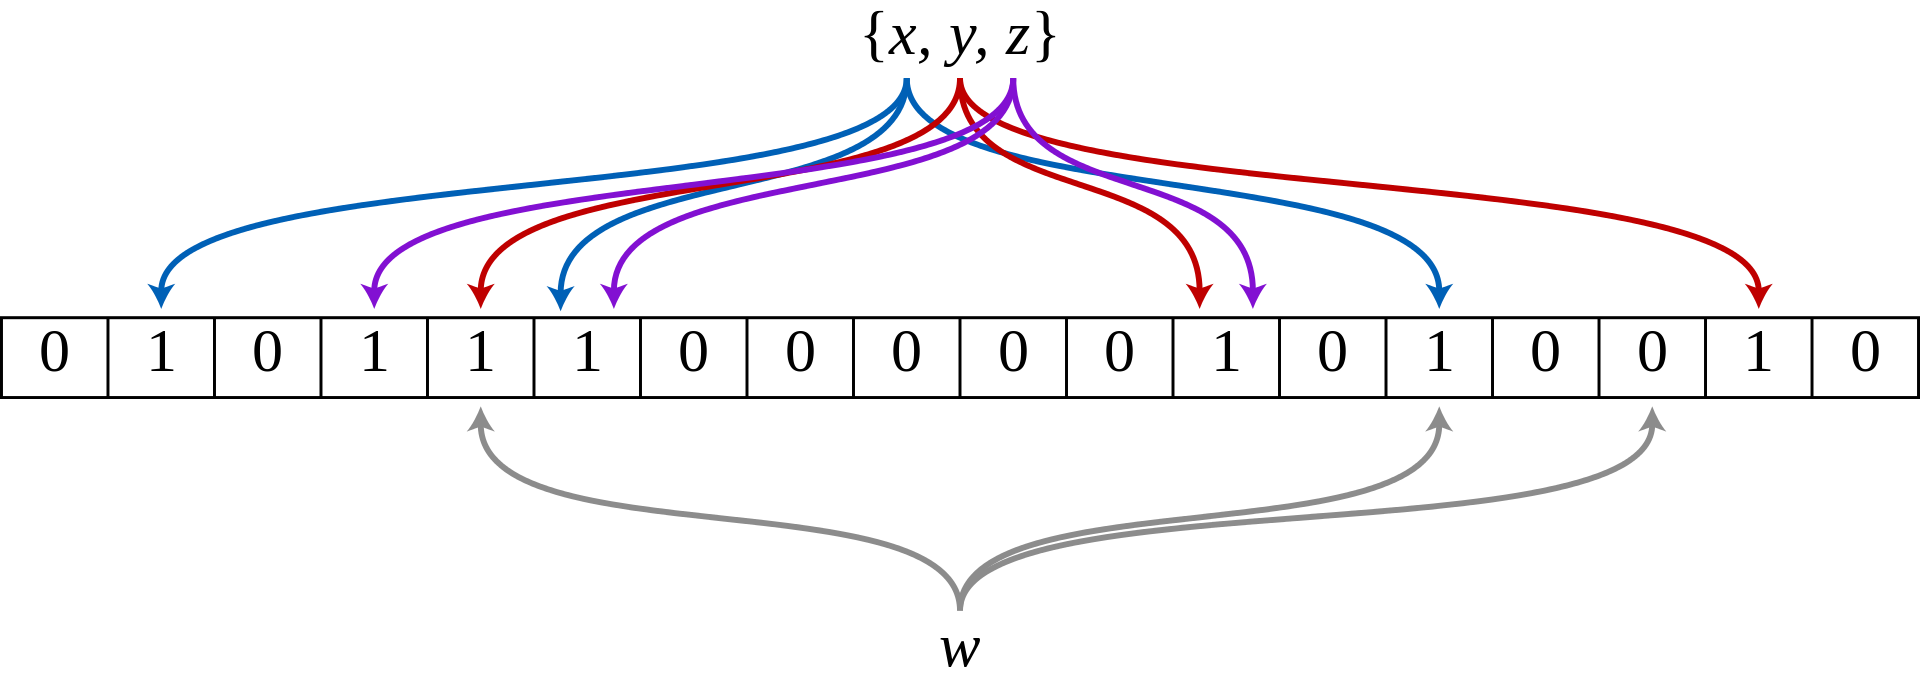
\includegraphics[width=\textwidth]{bloomfilter}
                \caption{Een bloomfilter, die de verzameling $\{x, y, z\}$ beschrijft. De logische OF met al deze elementen is al reeds uitgevoerd. De controle of $w$ ook in deze verzameling zit zegt dat deze er niet in zit, want een bit van de hashwaarde van $w$ in de bloomfilter is 0.}
                \label{fig:bloomfilter}
            \end{figure}
            \item We willen een verzameling van objecten in gehashte vorm bijhouden.
            \item Een Bloomfilter houdt de logische bitsgewijze OF bij van de hashwaarden van alle elementen.
            \item Om te weten of een object in de verzameling zit wordt deze eerst gehasht. Daarna wordt de logische EN operatie gebruikt op de bloomfilter met deze waarde.
            \item Als het resultaat verschilt van de hashwaarde dan zit het object er zeker niet in.
            \item Anders weten we het niet, en moet de verzameling doorzocht worden.
        \end{itemize}
        \item Men tracht de kans dat er een fout voorkomt zo klein mogelijk te maken.
    \end{enumerate}
\end{itemize}


\subsection{Het Karp-Rabinalgoritme}
\begin{itemize}
    \item Herleidt het vergelijken van strings tot het vergelijken van getallen.
    \item Aan elke mogelijke string die even lang is als $P$ wordt een getal toegekend.
    \item Er zijn $d^p$ verschillende strings met lengte $p$, zodat de getallen groot kunnen worden.
    \begin{itemize}
        \item Daarom worden de getallen beperkt tot deze die in één processorwoord (met lengte $w$ bits) voorgesteld kunnen worden, via een modulobewerking.
    \end{itemize}
    
    \item Meerdere strings zullen met hetzelfde getal moeten overeenkomen ($\equiv$ hashing).
    \item Gelijke strings betekent nog altijd gelijke getallen, maar een gelijk getal betekent niet meer dezelfde string.
    \begin{itemize}
        \item Bij een gelijk getal moet het patroon nog steeds vergeleken worden met de tekst op die positie.
    \end{itemize}
    \item Hoe worden de getallen gedefinieerd?
    \begin{itemize}
        \item Ze moeten in $O(1)$ berekend kunnen worden voor elk van de $O(t)$ deelstrings in de tekst.
        \item Een hashwaarde voor een string met lengte $p$ in $O(1)$ berekenen is niet realistisch.
        \item Daarom wordt de hashwaarde voor de deelstring op positie $j + 1$ berekend op basis van de deelstring op basis $j$.
        \item De eerste hashwaarde berekenen ($j = 0$) mag dan langer duren.
    \end{itemize}
    

    \item De voorstelling van $P$:
    \begin{itemize}
        \item We beschouwen een string als een getal in een $d-$tallig talstelsel omdat elk stringelement $d$ waarden kan aannemen zodat elk stringelement wordt voorgesteld door een cijfer tussen 0 en $d - 1$.
        
        $$H(P) = \sum_{i=0}^{p-1} P[i]d^{p-i-1} = P[0]d^{p-1} + P[1]d^{p-2} + \dots + P[p-2]d + P[p-1]$$

        \item Om de beperkte waarde te bekomen, wordt de rest bij deling door een getal $r$ (in de voorbeelden is $r = 29$) genomen. Dit wordt de \textbf{fingerprint} genoemd.
        $$H_r(P) = H(P)\;\mathrm{mod}\;r$$
    
        \item Dit is geen efficiënte operatie omdat de individuele getallen van de som in $H(p)$ groot kunnen worden, maar gelukkig
        $$(a + b) \;\mathrm{mod}\;r = (a\;\mathrm{mod}\;r + b\;\mathrm{mod}\;r)\;\mathrm{mod}\;r$$
    
        Dit geldt ook voor verschil en het product.
        \begin{itemize}
            \item Op deze manier wordt $H_r(P)$ als volgt gedefinieerd:
            $$H_r(P) = \sum_{i=0}^{p-1} P[i]d^{p-i-1}\;\mathrm{mod}\;r$$
            \alert In de voorbeelden wordt deze eigenschap niet gebruikt om het overzichtelijk te houden.
        \end{itemize}
    
        \item Omdat elk tussenresultaat nu binnen een processorwoord past, is $H_r(P)$ berekenen slechts $\Theta(p)$.

        
        \item Voor het alfabet $\Sigma = \{A, C, G, T\}$ gelden volgende waarden voor de stringelementen:
        \begin{table}[ht]
            \centering
            \begin{tabular}{c | c}
                A & 1 \\
                C & 2 \\
                G & 3 \\
                T & 4 
            \end{tabular}
        \end{table}
        \begin{align*}
            H(P) &= \sum_{i=0}^{8} P[i] \cdot 4^{8-i} \\
                 &= G\cdot 4^8 + C\cdot 4^7 + A\cdot 4^6 + G\cdot 4^5 + A\cdot 4^4 + G\cdot 4^3 + C\cdot 4^2 + A\cdot 4^1 + G\cdot 4^0\\
                 &= 3\cdot 4^8 + 2\cdot 4^7 + 1\cdot 4^6 + 3\cdot 4^5 + 1\cdot 4^4 + 3\cdot 4^3 + 2\cdot 4^2 + 1\cdot 4^1 + 3\cdot 4^0\\
                 &= 237031 \\
            H_r(P) &= 237031\;\mathrm{mod}\;29\\
                   &= 14
        \end{align*}
    \end{itemize}
    \item De voorstelling van $T$:
    \begin{itemize}
        \item De waarde $T_0$ bij beginpositie $j = 0$ wordt op dezelfde manier berekend als $P$.
        $$H(T_0) = \sum_{i=0}^{p-1} T[i]d^{p-i-1} = T[0]d^{p-1} + T[1]d^{p-2} + \dots + T[p-2]d + T[p-1]$$

        \item Er is nu een eenvoudig verband tussen het getal voor de deelstring $T_{j + 1}$ bij beginpositie $j + 1$ en dat voor $T_{j}$ bij beginpositie $j$:

        $$H(T_{j + 1}) = (H(T_j) - T[j]d^{p-1})d + T[j + p]$$

        \item Analoog aan $H_r(P)$ worden de waarden $H(T)$ ook modulo $r$ genomen, zodat $$H_r(T_{j + 1}) = H(T_{j + 1})\;\mathrm{mod}\;r$$

        (De waarde $T[j]d^{p-1}$ aftrekken en die van $T[j + p]$ optellen en er ook voor zorgen dat de macht die bij $T[j +1], T[j + 2], ... T[j + p -1]$  hoort met 1 verhoogt wordt door te vermenigvuldigen met $d$)

        \begin{table}[ht]
            \centering   
            \scalebox{0.4}{
                
            \begin{tabular}{|c|c c c c c c c c c c c c c c c c c c c c c c c cc |}
                    \hline
                    j & 0 & 1 & 2 & 3 & 4 & 5 & 6 & 7 & 8 & 9 & 10 &11&12 &13 &14 &15 &16 &17 &18 &19 &20 &21 &22 &23&24\\    
                    T & G & C & A & T & C & G & C & A & G & A & G&C & A & G & A & G & T & A & C & A & G & C & A & C & G\\
                  \hline
                  $H(T_j)$ & 238311 & 166813  & 142967 & 309726 & 190329 &  237031& 161693 & 122487  & 227808  & 124801  & 237062  & 161817  & 122983  & 229790  & 132729  & 268774  & 26523  &  / & /  &/   &/   &/   &/&/ &/ \\
                  $H_r(T_j)$ & \nm{18} & \nm{5}  & \nm{26}  & \nm{6} & \nm{2} & \um{14} & \nm{18}  & \nm{20}  & \nm{16}  & \um{14}  & \nm{16}  & \nm{26}  & \nm{23}  &\nm{23}   &\nm{25}   & \nm{2}  & \nm{17}  & /  &/   & /  & /  & /  &/& /&/ \\
                  \hline
                  $H(T_0)$ & \multicolumn{25}{l|}{$3\cdot 4^8 + 2\cdot 4^7 + 1\cdot 4^6 + 4\cdot 4^5 + 2\cdot 4^4 + 3\cdot 4^3 + 2\cdot 4^2 + 1\cdot 4^1 + 3\cdot 4^0 = 238311$}   \\
                  $H(T_1)$ & \multicolumn{25}{l|}{$\big(H(T_0) - T[0]\cdot 4^8\big)\cdot 4 + T[9] = (238311 - 3\cdot 4^8)\cdot 4 + 1 = 166813$}   \\
                  $H(T_2)$ & \multicolumn{25}{l|}{$\big(H(T_1) - T[1]\cdot 4^8\big)\cdot 4 + T[10] = (166813 - 2\cdot 4^8)\cdot 4 + 3 = 142967$}   \\
                  $H(T_3)$ & \multicolumn{25}{l|}{$\big(H(T_2) - T[2]\cdot 4^8\big)\cdot 4 + T[11] = (142967 - 1\cdot 4^8)\cdot 4 + 2 = 309726$}   \\
                  $H(T_4)$ & \multicolumn{25}{l|}{$\big(H(T_3) - T[3]\cdot 4^8\big)\cdot 4 + T[12] = (309726 - 4\cdot 4^8)\cdot 4 + 1 = 190329$}   \\
                  $H(T_5)$ & \multicolumn{25}{l|}{$\big(H(T_4) - T[4]\cdot 4^8\big)\cdot 4 + T[13] = (190329 - 2\cdot 4^8)\cdot 4 + 3 = 237031$}   \\
                  $H(T_{j})$ & \multicolumn{25}{c|}{$\cdots$}   \\
                  \hline   
                  $P$ & G&C&A&G&A&G&C&A&G&\multicolumn{16}{c|}{} \\
                  $T[5\cdots 13]$ &\m{G}&\m{C}&\m{A}&\m{G}&\m{A}&\m{G}&\m{C}&\m{A}&\m{G}&\multicolumn{16}{c|}{} \\
                  $T[9\cdots 17]$ &\nm{A}&G&C&A&G&A&G&T&A&\multicolumn{16}{c|}{} \\
                  \hline   
            \end{tabular}
            }
            \caption{Het Karp-Rabinalgoritme.}
        \end{table}

       
    \end{itemize}
        

        \item Het berekenen van $H_r(P)$, $H(T_0)$ en $d^{p-1}\;\mathrm{mod}\;r$ vereist $\Theta(p)$ operaties.
        \item Het berekenen van alle andere fingerprints $H_r(T_j) (0 < j \leq t - p)$ vergt $\Theta(t)$ operaties.
        \item Dit is $\Theta(t + p)$.
        \item Maar, de strings moeten nog vergeleken worden als de fingerprints hetzelfde zijn.
        \item In het slechtste geval zijn de fingerprints op elke positie gelijk, zodat de totale performantie $\textbf{O(tp)}$ is.
        \item Er zijn nu nog twee mogelijkheden om $r$ te bepalen:
        \begin{enumerate}
            \item \textbf{Vaste $r$}
            \begin{itemize}
                \item Kies $r$ als een zo groot mogelijk priemgetal zodat $rd \leq 2^w$.
                \item Priemgetallen zorgt ervoor dat gelijkaardige deelstrings dezelfde fingerprinters zouden opleveren.
                \item Een groot priemgetal zorgt voor een groot aantal mogelijke fingerprints.
                \item Er is nu wel een nieuw verband tussen $H_r(T_{j + 1})$ en $H_r(T_j)$:
                $$H_r(T_{j + 1}) = \bigg(\big((H_r(T_j) + r(d - 1) - T[j](d^{p-1}\;\mathrm{mod}\;r)) \;\mathrm{mod}\;r\big)d + T[j + 1] \bigg)\;\mathrm{mod}\;r$$
                
                (De term $r(d - 1)$ wordt toegevoegd om een negatief tussenresultaat te vermijden.)
            \end{itemize}


            \item \textbf{Random $r$}
            \begin{itemize}
                \item Soms is een vaste $r$ nadelig: er kan bijvoorbeeld een slechte waarde gekozen worden.
                \item De veiligste implementatie gebruikt een willekeurige priem $r$ uit een bepaald bereik.
                \item Een groter bereik reduceert de kans op fouten.
                \item Het aantal priemgetallen kleiner of gelijk aan $k$ is $\frac{k}{\ln k}$.
                \item Door $k$ groot te kiezen zal slechts een klein deel van die priemgetallen een fout veroorzaken.
                \item De kans dat $r$ één van die priemen is wordt klein.
                \item Voor $k = t^2$ is de kans op één enkele foute $O(1/t)$.
                \item Om fouten helemaal te vermijden zijn er twee mogelijkheden:
                \begin{itemize}
                    \item Overgaan naar een andere methode als de fout gesignaleerd wordt.
                    \item Herbeginnen met een nieuwe random priem $r$.
                \end{itemize}
            \end{itemize}
        \end{enumerate}

    

\end{itemize}


\subsection{Zoeken met automaten}
\begin{itemize}
    \item Een \textbf{automaat} is een informatieverwerkend eenheid.
\end{itemize}
\subsubsection{Deterministische automaten}    
\begin{itemize}
     \item Een deterministische automaat (DA) bestaat uit: 
    \begin{itemize}
        \item Een eindige verzameling invoersymbolen $\Sigma$.
        \item Een eindige verzameling staten $S$.
        \item Een begintoestand $s_0 \in S$.
        \item Een eindige verzameling eindstaten $F \subset S$.
        \item Een overgangsfunctie $p(t, a)$ die de nieuwe toestand geeft wanneer de DA in toestand $t$ invoersymbool $a$ ontvangt.
    \end{itemize}
    \item Een DA kan voorgesteld worden een gelabelde multigraaf $G$.
    \begin{itemize}
        \item De knopen zijn de toestanden.
        \item De verbindingen zijn de overgangen.
    \end{itemize}
    \item Als de DA zich in een eindstaat bevindt na het invoeren van een string, dan wordt deze string herkent door de DA.
    \item Een taal die door een DA herkent wordt is regulier.
    \begin{itemize}
        \item Dit is de verzameling van labels $P_G(\{s_0\}, F)$
    \end{itemize}
\end{itemize}
\subsubsection{Niet-deterministische automaten}    
\begin{itemize}
     \item Een niet-deterministische automaat (NA) bestaat uit:
     \begin{itemize}
         \item Een eindige verzameling invoersymbolen $\Sigma$.
         \item Een eindig aantal statenbits. De verzameling van statenbits die de waarde 1 hebben is de staat van de NA.
         \item Een beginbit $b_0$ en een verzameling eindbits.
         \item De overgangsfunctie $s(i, a)$ is de verzameling statenbits die een signaal krijgen van statenbit $i$ als de inkomende letter $a$ is. Een statenbit dat een signaal binnenkrijgt krijgt de waarde 1.
         \item Nul of meerdere $\epsilon$-overgangen. Een $\epsilon$-overgang van statenbit $i$ naar statenbit $j$ zorgt ervoor dat wanneer $i$ een signaal binnenkrijgt, dit signaal direct doorstuurt naar $j$.
     \end{itemize}
     \item Een NA herkent een string als op het einde van die string er één of meer eindbits aan staan.
\end{itemize}

\subsubsection{De deelverzamelingconstructie}
\begin{itemize}
    \item Een NA is een alternatieve voorstelling van een DA.
    \item Elke NA kan omgezet worden in een DA.
    \begin{itemize}
        \item Een DA is eenvoudiger om te implementeren: de nieuwe toestand wordt opgezocht in een tweedimensionale tabel.
    \end{itemize}
    \item Elke staat van de NA komt overeen met een verzameling statenbits die aanstaan.
    \item Als er $k$ statenbits zijn, dan zijn er $2^k$ mogelijke deelverzamelingen.
    \begin{itemize}
        \good Slechts een klein aantal van deze deelverzamelingen worden effectief bereikt.
    \end{itemize}
    \item Er is een impliciet gegeven multigraaf met $2^k$ knopen.
    \item Om een DA te construeren zijn er twee hulpoperaties nodig:
    \begin{enumerate}
        \item \textbf{$\epsilon$-sluiting($T$)}: De deelverzameling van statenbits bereikbaar via $\epsilon$-overgangen vanuit een verzameling statenbits $T$.
        \item \textbf{$p(T, a)$}: De deelverzameling van statenbits rechtstreeks bereikbaar vanuit een toestand $t$ uit $T$ voor het invoersymbool $a$.
    \end{enumerate}
    \item Om een DA te construeren moet er een verzameling van toestanden $S$ met begin- en eindtoestanden en een overgangstabel $M$ opgesteld worden.
    \begin{itemize}
        \item De begintoestand is $\epsilon$-sluiting($b_0$).
        \item Elke andere staat wordt bekomen door $\epsilon$-sluiting$(p(T, a))$ voor elke andere staat $T$ en invoersymbool $a$.
        \item Een eindtoestand van de DA bevat minstens één eindtoestand van de NA.
        Vervolgens wordt voor elke toestand $T$ de overgang voor elk invoersymbool $a$ bepaald.
    \end{itemize}
    \item Figuur \ref{fig:deelverzameling1} toont de DA geconstrueerd uit de NA van figuur \ref{fig:thompson3}.
    \begin{figure}[ht]
        \centering
        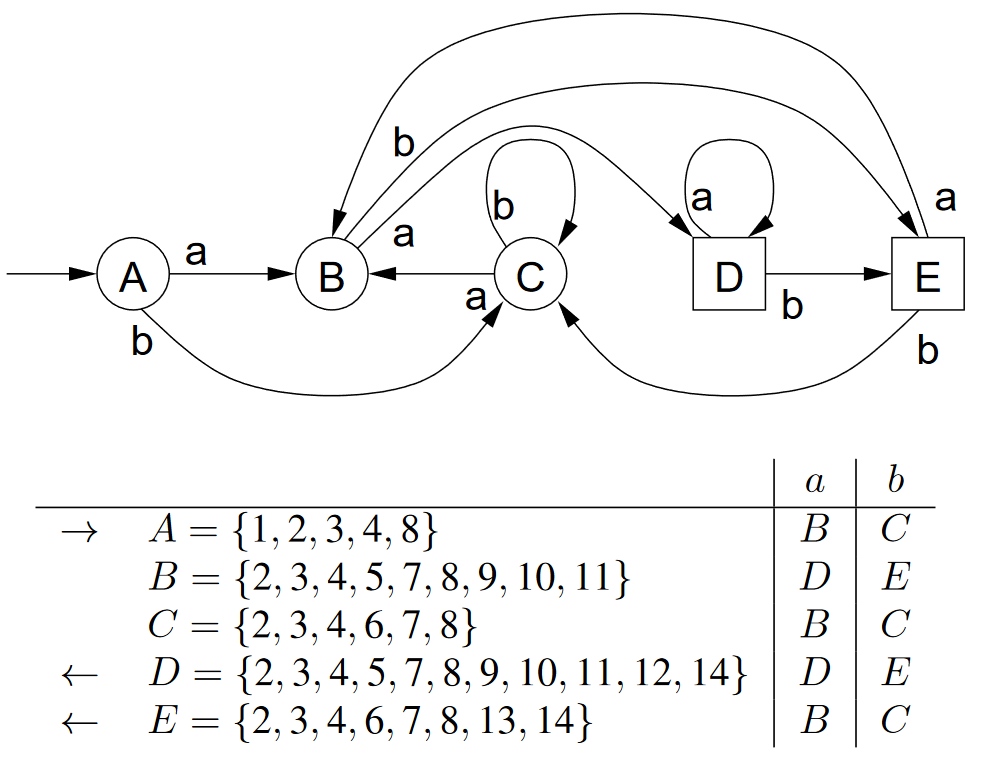
\includegraphics[width=0.75\textwidth]{deelverzameling1}
        \caption{Deterministische automaat geconstrueerd uit de NA van figuur \ref{fig:thompson3}.}
        \label{fig:deelverzameling1}
    \end{figure}
\end{itemize}

\subsubsection{Automaten voor regexps}
\begin{itemize}
    \item Een reguliere taal kan herkend worden door een DA of NA.
    \item Een NA kan opgebouwd worden vanuit een regexp door de \textbf{constructie van Thompson}.
    \begin{itemize}
        \item Er worden NA's gedefinieerd voor basiselementen van een regexp: elk element uit $\Sigma$ en $\epsilon$ (figuur \ref{fig:thompson1}).
        \begin{figure}[ht]
            \centering
            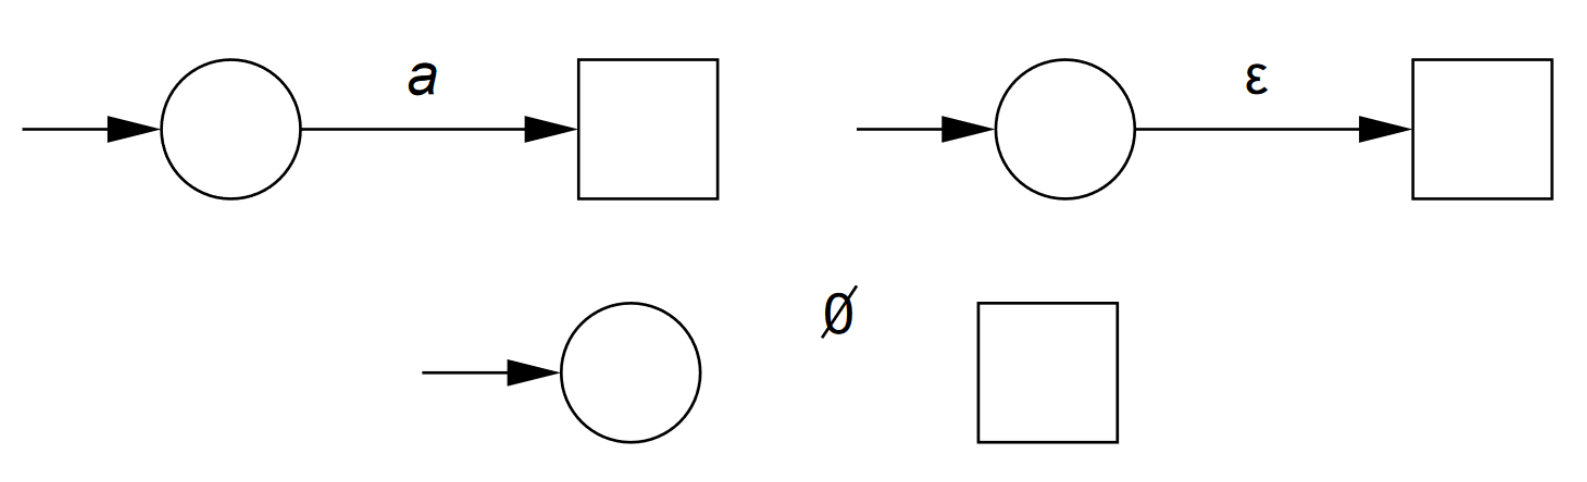
\includegraphics[width=0.7\textwidth]{thompson1}
            \caption{Constructie van Thompson: basiselementen.}
            \label{fig:thompson1}
        \end{figure}
        \item Deze NA's kunnen samengesteld worden voor elk van de drie basisoperatoren: unie, concatenatie en Kleenesluiting (figuur \ref{fig:thompson2}).
        \begin{figure}[ht]
            \centering
            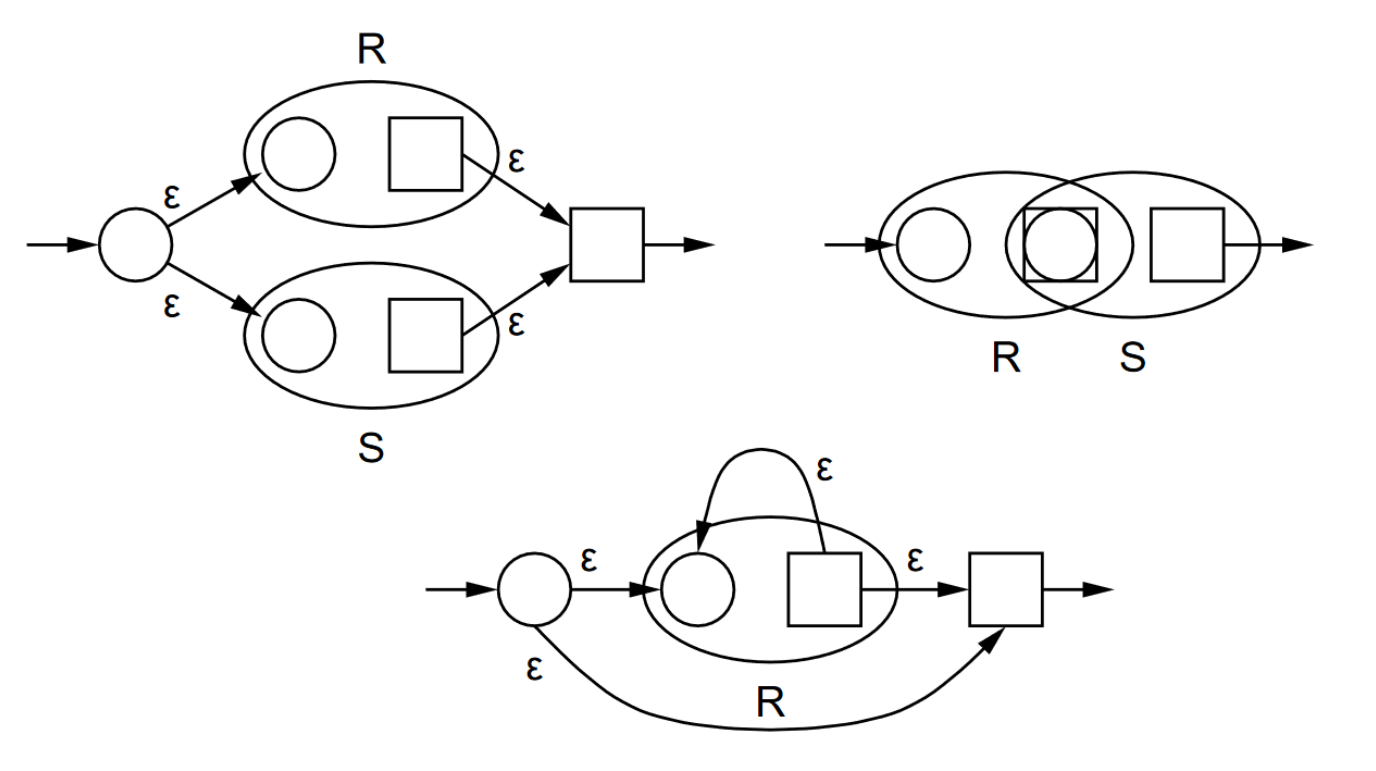
\includegraphics[width=0.7\textwidth]{thompson2}
            \caption{Constructie van Thompson: unie, concatenatie en Kleenesluiting.}
            \label{fig:thompson2}
        \end{figure}
    \end{itemize}
    \item Een NA die op deze manier geconstrueerd is, zal alle strings genereerd door de regexp herkennen en geen andere.
    \item Figuur \ref{fig:thompson3} toont de NA bekomen met deze constructie voor de regexp $(a|b)*a(a|b)$.
    \begin{figure}[ht]
        \centering
        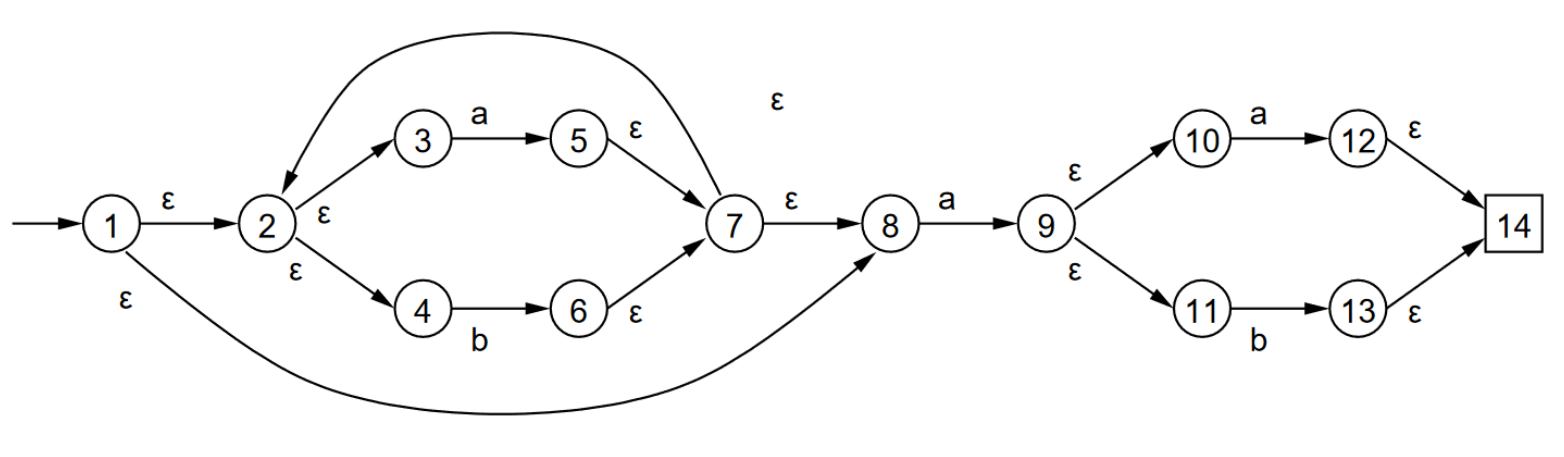
\includegraphics[width=\textwidth]{thompson3}
        \caption{Constructie van Thompson: NA voor $(a|b)*a(a|b)$.}
        \label{fig:thompson3}
    \end{figure}
    \item Een NA uit de constructie van Thompson heeft drie eigenschappen:
    \begin{itemize}
        \item Er is slechts één beginbit en één eindbit.
        \item Het aantal bits is niet groter dan tweemaal het aantal elementen in de regexp.
        \item Vanuit elke bit vertrekken er hoogstens twee overgangen: ofwel één overgang voor een symbool uit $\Sigma$, ofwel hoogstens twee $\epsilon$-overgangen.
    \end{itemize}
    \item \textbf{Stelling 2} Een taal kan herkend worden door een eindige deterministische automaat als en slechts als ze regulier is.
    \item \textbf{Bewijs:}
    \begin{itemize}
        \item Een taal die herkend wordt door een automaat is zeker regulier.
        \begin{itemize}
            \item Een taal bestaande uit labels van de paden vertrekkend uit een beginstaat en eindigd in een eindstaat is steeds regulier.
        \end{itemize}
        \item Als een taal regulier is, kan ze beschreven worden door een regexp en voor deze regexp kan eerst een NA opgebouwd worden, en vervolgens tot een DA omgevormd worden via de deelverzamelingconstructie.
    \end{itemize}
    \item \textbf{Gevolg:}
    \begin{itemize}
        \item Niet alle contextvrije talen zijn regulier.
        \begin{itemize}
            \item Stel de strings beginnend met een aantal 'a's gevolgd door evenveel 'b's
            \item Als er een 'b' tegengekomen wordt, moet er ergens bijgehouden worden hoeveel 'a's er al zijn geweest.
            \item Dit aantal is niet begrensd en kan niet vooraf in een eindig geheugen geplaatst worden.
        \end{itemize}
    \end{itemize}
\end{itemize}

\subsubsection{Minimalisatie van een automaat}



\subsection{De Shift-AND-methode}
\begin{itemize}
    \item Bitgeoriënteerde methode, die zeer efficiënt werkt voor \textbf{kleine patronen}.
    \item Hou voor elke positie $j$ in $T$ bij welke prefixen van $P$ overeenkomen met de tekst, eindigend op $j$.
    \item Er is een tabel $S$ met $d$ woorden (tabel \ref{table:shiftandS}). Een bit $i$ van woord $S[s]$ is waar als karakter $s$ op plaats $i$ in $P$ voorkomt.
    \begin{table}[ht]
        \centering
        \begin{tabular}{l | c c c c c c c c c}
            & G & C & A & G & A & G & C & A & G \\
            \hline
            S['A'] & 0 & 0 & \textbf{1} & 0 & \textbf{1} & 0 & 0&\textbf{1} & 0 \\
            S['C'] & 0 & \textbf{1} & 0 & 0 & 0 & 0 & \textbf{1} & 0 & 0\\
            S['G'] & \textbf{1} & 0 & 0 & \textbf{1} & 0 & \textbf{1} & 0 & 0 & \textbf{1} \\
            S['T'] & 0 & 0 & 0 & 0 & 0 & 0 & 0 & 0& 0\\
        \end{tabular}
        \caption{De tabel $S$ bevat een bitpatroon voor elk karakter $s$ in het alfabet. Karakters die niet in het patroon voorkomen krijgen een bitpatroon bestaande uit $p$ nulbits.} 
        \label{table:shiftandS}
    \end{table}
    \item Een tabel $R_j$ van $p$ logische waarden geeft voor het $i$-de element het prefix van lengte $i$, die hoort bij tekstpositie $j$.
    %\item In totaal zijn er $t$ van deze $R_j$ tabellen (tabel \ref{table:shiftandR}).

    \begin{table}[ht]
        \centering
        \scalebox{0.6}{
        
        \begin{tabular}{|c c | c c c c c c c c c c c c c c c c c c c c c c c c c |}
            \hline
            $R_j$& & $R_0$&$R_1$&$R_2$&$R_3$&$R_4$&$R_5$&$R_6$&$R_7$&$R_8$&$R_9$&$R_{10}$&$R_{11}$&$R_{12}$&$R_{13}$&$R_{14}$&$R_{15}$&$R_{16}$&$R_{17}$&$R_{18}$&$R_{19}$&$R_{20}$&$R_{21}$&$R_{22}$&$R_{23}$&$R_{24}$\\
            & T& G & C & A & T & C & G & C & A & G & A & G&C & A & G & A & G & T & A & C & A & G & C & A & C & G\\
            \hline
            $R[0]$ & G & \textbf{1}&0&0&0&0& \textbf{1}&0&0& \textbf{1}&0& \textbf{1}&0&0& \textbf{1}&0& \textbf{1}&0&0&0&0& \textbf{1}&0&0&0& \textbf{1}  \\
            $R[1]$ & C & 0&\textbf{1}&0&0&0&0& \textbf{1}&0&0&0&0& \textbf{1}&0&0&0&0&0&0&0&0&0& \textbf{1}&0&0&0  \\
            $R[2]$ & A & 0&0&\textbf{1}&0&0&0&0& \textbf{1}&0&0&0&0& \textbf{1}&0&0&0&0&0&0&0&0&0& \textbf{1}&0&0  \\
            $R[3]$ & G & 0&0&0         &0&0&0&0&0& \textbf{1}&0&0&0&0& \textbf{1}&0&0&0&0&0&0&0&0&0&0&0  \\
            $R[4]$ & A & 0&0&0         &0&0&0&0&0&0& \textbf{1}&0&0&0&0& \textbf{1}&0&0&0&0&0&0&0&0&0&0  \\
            $R[5]$ & G & 0&0&0         &0&0&0&0&0&0&0& \textbf{1}&0&0&0&0& \textbf{1}&0&0&0&0&0&0&0&0&0  \\
            $R[6]$ & C & 0&0&0         &0&0&0&0&0&0&0&0& \textbf{1}&0&0&0&0&0&0&0&0&0&0&0&0&0  \\
            $R[7]$ & A & 0&0&0         &0&0&0&0&0&0&0&0&0& \textbf{1}&0&0&0&0&0&0&0&0&0&0&0&0  \\
            $R[8]$ & G & 0&0&0         &0&0&0&0&0&0&0&0&0&0& \m{1}&0&0&0&0&0&0&0&0&0&0&0  \\

            \hline
        \end{tabular}
        }
        \caption{De opeenvolgende tabellen $R_j$. Er moet slechts één tabel in het geheugen bijgehouden worden, en dat is die op het huidige karakterpositie $j$.}
        \label{table:shiftandR}
    \end{table}

    \begin{itemize}
        \item De startabel $R_0$ wordt opgebouwd als $R_0[0] = 1$ en $R_0[1\;\cdots\;p - 1] = 0$.
        \item Opeenvolgende tabellen $R_{j + 1}$ kunnen via efficiënte bitoperaties bekomen worden:
        $$R_{j + 1} = \hbox{Schuif}(R_j) \hbox{ EN } S[T[j + 1]]$$
        \item De schuif-operatie verschuift een bitpatroon naar rechts, en voegt links een éénbit toe.
    \end{itemize}

    \item Het patroon wordt gevonden in de tekst op positie $j - p$ als $R_j[p - 1] = 1$.

    \item Er zijn ook \textbf{benaderingen mogelijk}. Deze benaderingen maken gebruik van dezelfde tabel $R_j = R^0_j$, en een nieuwe tabel $R^1_j$, waarvan de definitie afhankelijk is van het soort benadering. 
    \begin{itemize}
        \item \textbf{Karakters inlassen} 
        \begin{itemize}
            \item De tabel $R^1_j$ duidt alle prefixen aan eindigend op positie $j$ met hoogstens één inlassing.
            $$R^1_{j + 1} = R^0_j \hbox{ OF }(\hbox{Schuif}(R_j) \hbox{ EN } S[T[j + 1]]) $$
        \end{itemize}
        \item \textbf{Karakters verwijderen} 
        \begin{itemize}
            \item De tabel $R^1_j$ duidt alle prefixen aan eindigend op positie $j$  met hoogstens één verwijdering.
            $$R^1_{j + 1} = \hbox{Schuif}(R^0_{j+1}) \hbox{ OF }(\hbox{Schuif}(R_j) \hbox{ EN } S[T[j + 1]]) $$
        \end{itemize}
        \item \textbf{Karakters vervangen}
        \begin{itemize}
            \item De tabel $R^1_j$ duidt alle prefixen aan eindigend op positie $j$ waarbij $i - 1$ van de eerste $i$ karakters van $P$ overeenkomen met $i - 1$ karakters van de $i$ karakters die in de tekst eindigen bij positie $j$.
            $$R^1_{j + 1} = \hbox{Schuif}(R^0_{j}) \hbox{ OF }(\hbox{Schuif}(R_j) \hbox{ EN } S[T[j + 1]]) $$
        \end{itemize}
    \end{itemize}
\end{itemize}

